%% Title and Preprocessing
\documentclass[titlepage]{article}\pagestyle{empty}
\usepackage{amsmath}

\author{Kevin Fang}
\title{Homework \#5}
\date{\today}
\usepackage[left=1cm, right=2cm, vmargin=1cm]{geometry}
\usepackage{amsfonts}

\def\therefore{\boldsymbol{\text{ }
\leavevmode
\lower0.4ex\hbox{$\cdot$}
\kern-.5em\raise0.7ex\hbox{$\cdot$}
\kern-0.55em\lower0.4ex\hbox{$\cdot$}
\thinspace\text{ }}}

\usepackage{mathtools}
\DeclarePairedDelimiter\ceil{\lceil}{\rceil}
\DeclarePairedDelimiter\floor{\lfloor}{\rfloor}

% Start Document Here
\begin{document}
\maketitle

\pagebreak
\section*{Question 3.} Solve the following sections from the Discrete Math zyBook:
\subsection*{(a): Exercise 4.1.3} 
\subsubsection*{B.} Not a function and fails for $x = 2$ and $x = -2$.
\subsubsection*{C.} Is a function for all of $\mathbb{R}$. The range of the function is $[0,\infty)$.
\subsection*{(b): Exercise 4.1.5} 
\subsubsection*{B.} 
$\{4,9,16,25\}$
\subsubsection*{D.}
$\{0, 1, 2, 3, 4, 5\}$
\subsubsection*{H.} 
$A \times A = \{(1,1),(1,2),(1,3),(2,1),(2,2),(2,3),(3,1),(3,2),(3,3)\}$.
\subsubsection*{I.} 
$A \times A = \{(1,2),(1,3),(1,4),(2,2),(2,3),(2,4),(3,2),(3,3),(3,4)\}$.
\subsubsection*{L.} 
$\{\emptyset, \{2\}, \{3\}, \{2, 3\}\}.$

\pagebreak
\section*{Question 4.}
\subsection*{I - Solve the following sections from the Discrete Math zyBook} 
\subsubsection*{(a): 4.2.2}
\subsubsection*{C.}
One to one but not onto.\\
For $h(x) = 2$, there does not exist an $x \in Z$ such that $h(x) = 2$.\\
\subsubsection*{G.}
One to one but not onto.\\
For $f(x, y) = (0, 1)$, there does not exist a pair of $(x, y) \in Z \bigtimes Z$ such that $f(x, y) = (0, 1)$.\\
\subsubsection*{K.}
Neither one to one or onto.\\
For $f(1, 3) = 5$ and $f(2, 1) = 5$, there exist a value in the range such that its values of the domain are different.\\
For $f(x, y) = 1$ or $f(x, y) = 2$,  there does not exist a pair of $(x, y) \in Z^+ \bigtimes Z^+$ such that $f(x, y) = 1$ or $f(x, y) = 2$.\\
\subsubsection*{(b): 4.2.4}
\subsubsection*{B.}
Neither one to one or onto.\\
For $f(000) = 100$ and $f(100) = 100$, there exist a value in the range such that its values of the domain are different.\\
For $f(x) = 000$, there does not exist a $x \in \{0, 1\}^3$ such that $f(x) = 000$.\\
\subsubsection*{C.}
One to one and onto.\\
\subsubsection*{D.}
One to one but not onto.\\
For $f(x) = 0001$, there does not exist a $x \in \{0, 1\}^3$ such that $f = 0001$.\\
\subsubsection*{G.}
Neither one to one or onto.\\
For $X_1 = \{2\}$ and $X_2 = \{1, 2\}$ where $F(X_1) = F(X_2) = \{2\}$, there exist a value in the range such that its values of the domain are different.\\
There does not exist a $X$ in the domain such that the value in the range is $\{1\}$.\\
\subsection*{II - Give an example of a function from the set of integers to the set of positive integers that is: }  
\subsubsection*{A:}
$f(x) = 2x$ for $x \ge 0$ and $2|x|+1$ for $x < 0$.
\subsubsection*{B:}
$f(x) = |x|$.
\subsubsection*{C:}
$f(x) = 2x$ for $x \ge 0$ and $2|x|-1$ for $x < 0$.
\subsubsection*{D:}
$f(x) = 99$.

\pagebreak
\section*{Question 5.} Solve the following sections from the Discrete Math zyBook:
\subsection*{(a): Exercise 4.3.2} 

\subsubsection*{C.} 
This function is well defined.\\
$f^{-1}(x)=\frac{x-3}{2}$.
\subsubsection*{D.} 
$f(x)$ is not one to one. \\
$f^{-1}(x)$ is not well defined.
\subsubsection*{G.} 
This function is well defined.\\
Both reverse the input bits. 
\subsubsection*{I.} 
This function is well defined.\\
$f^{-1}(x,y) = (x - 5, y+2)$.

\subsection*{(b): Exercise 4.4.8}
\subsubsection*{C.} $f \circ h(x) = 2x^2 + 5$
\subsubsection*{D.} 
$h \circ f(x) = (2x + 3)^2 + 1$\\
$h \circ f(x) = 4x^2 + 12x + 10$

\subsection*{(c): Exercise 4.4.2}
\subsubsection*{B.} 
$f \circ h(52) = (\ceil*{52/5})^2 =  11^2 = 121$
\subsubsection*{C.} 
$g \circ h \circ f(4) = 2^{(\ceil*{(4^2)/5})} = 2^{(\ceil*{(16/5})} = 2^4 = 16$

\subsubsection*{D.} 
$h(f(x))=\ceil*{\frac{x^2}{5}}$
\subsection*{(d): Exercise 4.4.6}
\subsubsection*{C.} $h(f(010))=111$
\subsubsection*{D.} Range is $\{101, 111\}$.
\subsubsection*{E.} Range is $\{001, 011, 101, 111\}$.

\subsection*{(E): Exercise 4.4.4}
\subsubsection*{C.}
No.
When $f$ is not one-to-one, there exist a value in the range such that its values of the domain are different.\\
$g \circ f(x_1) = g(f(x_1)) = g(y)$\\
$g \circ f(x_2) = g(f(x_2)) = g(y)$\\
This indicate that $g \circ f$ exist a value in the range such that its values of the domain are different.\\
\subsubsection*{D.}
Yes.
See Figrue 1: Exercise 4.4.4.D.
\begin{figure}
    \centering
    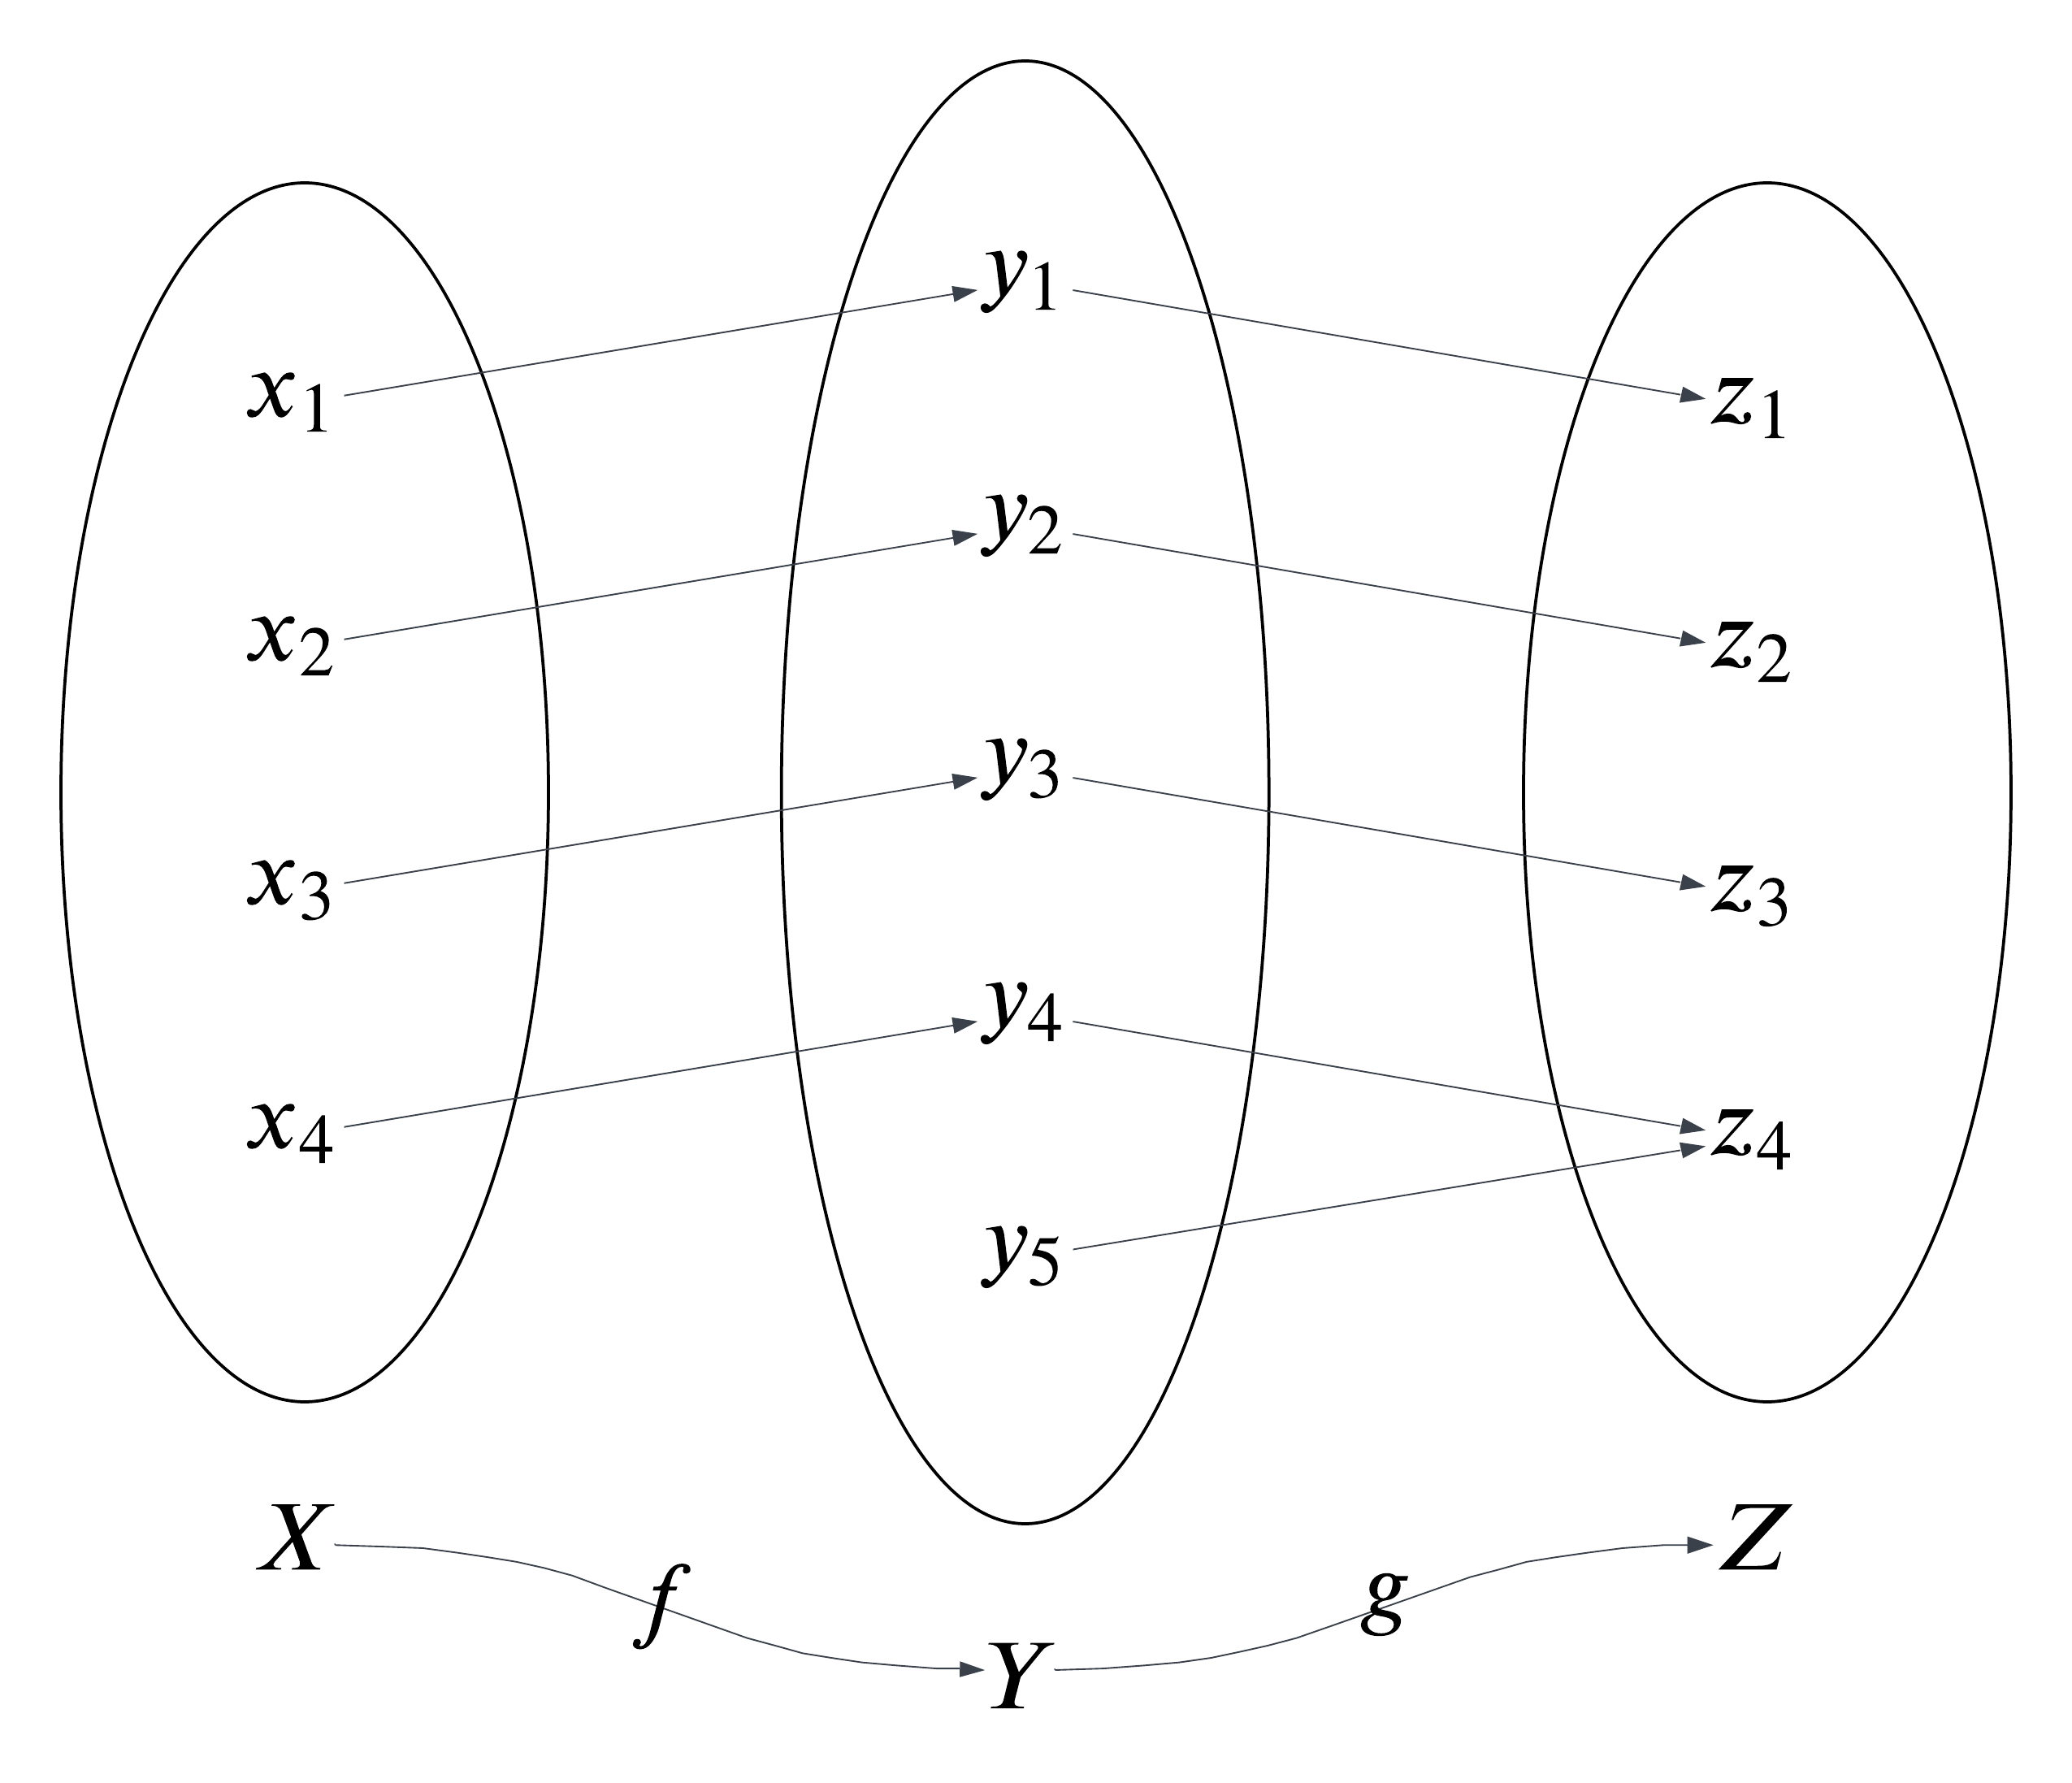
\includegraphics[width=1\linewidth]{Exercise 4.4.6.D.png}
    \caption{Exercise 4.4.4.D}
    \label{fig:enter-label}
\end{figure}

\end{document}